\section{Modelos}
\begin{frame}
% \blfootnote{\footcite{aggarwal_recommender_2016}}
\begin{itemize}
    \item<1-> \textbf{Basado en contenido}\onslide<3->{: PLN del texto de las propuestas}
    \item<2-> \textbf{Basado en filtrado colaborativo}\onslide<3->{: Graph Neural Networks (LightGCN)}
    \item<4-> \textbf{Híbrido}: Ensamblaje de los dos anteriores
    % \item<5-> \color{gray}{\textbf{Basado en conocimiento}: No hecho\footnote{\footcite{valiente_integration_2022}}}
\end{itemize}
\end{frame}

\subsection{Modelo basado en contenido}
\begin{frame}{Definición}
    TODO: Figura que muestre un ``espacio" 2d o 3d representando los embeddings de las propuestas, y ahí justo en el medio un icono del usuario
\end{frame}

\begin{frame}{Resultados}
    \begin{figure}
        \centering
        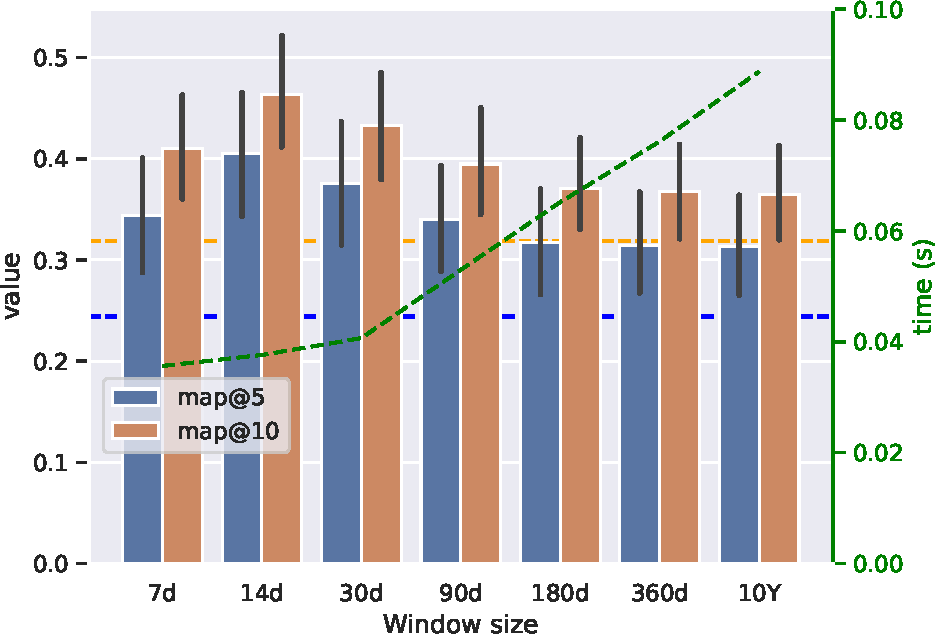
\includegraphics[height=45mm]{./images/graphs/11_cosine_results_window-size_W-THU_normalize=True.pdf}
        \caption{Rendimiento del modelo PLN con respecto al tamaño de la ventana de entrenamiento}
    \end{figure}
\end{frame}

\subsection{Modelo basado en filtrado colaborativo}
\begin{frame}{Definición}
    TODO: ¿Pongo la formula de los embeddings y la agregación? Yo creo que sí, la figura del paper también tá chula.
\end{frame}

\begin{frame}{Fine-tuning de LightGCN I}
\begin{table}[]
    \centering
    \begin{tabular}{l|c|c}
\textbf{Hiperparámetro} & \textbf{Valores} & \textbf{Muestreo} \\
\hline
Embedding dim. & $1\leq e\leq 1024, e\in \mathbb{N}$ & Loguniforme \\
Convolution layers & $c\in \{1,2,3,4,5,6\}$ & Uniforme \\
Batch size & $bs\in\{64,128,256,512,1024\}$ & Uniforme \\
Learning rate & $10^{-4}\leq lr\leq 1, lr\in \mathbb{R}$ & Loguniforme \\
L2 regularization & $10^{-7}\leq l2 \leq 10^{-2}, l2 \in \mathbb{R}$ & Loguniforme \\
    \end{tabular}
    \caption{Espacio de búsqueda de hiperparámetros para LightGCN}
\end{table}
\blfootnote{\footcite{bergstra_making_2013}}
\blfootnote{\footcite{liaw_tune_2018}}
\end{frame}

\begin{frame}{Fine-tuning de LightGCN II}
    TODO: Aquí pondré alguna figura que ejemplifique el problema de hyperoptimizar conociendo el futuro o algo así
\end{frame}

\begin{frame}{Fine-tuning de LightGCN III}
    TODO: Aquí pondre como una especie de ``progress bar" que se rellene con distintos colores para indicar la parte que se usa para elegir los hiperparámetros y la que se testea como ``modelo realista''
\end{frame}

\begin{frame}{Resultados GNN}
\begin{columns}
\column{.5\linewidth}
\begin{figure}
    \centering
    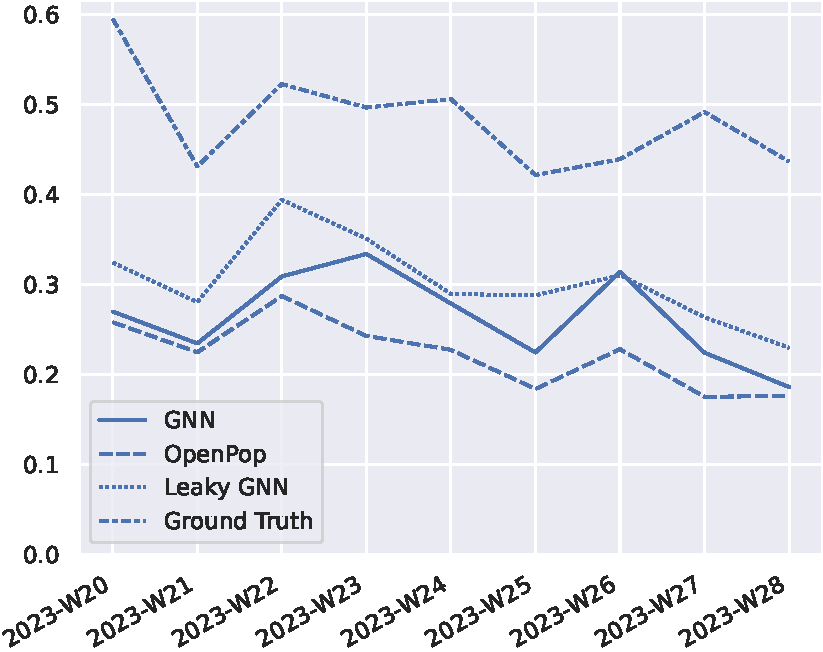
\includegraphics[height=45mm]{./images/graphs/09_gnn_results_precision_5_leaky.pdf}
    \caption{precision@5 del modelo GNN}
\end{figure}
\column{.5\linewidth}
\begin{figure}
    \centering
    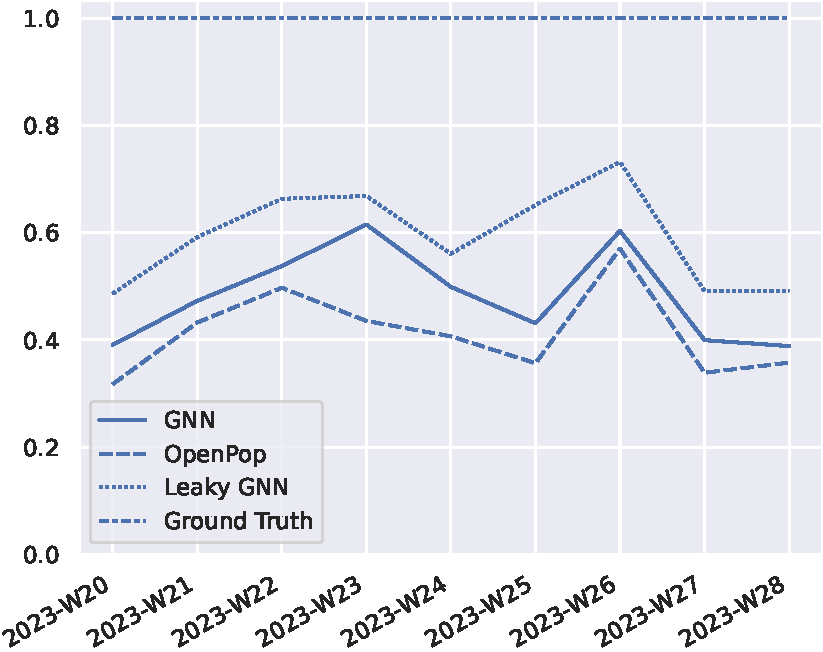
\includegraphics[height=45mm]{./images/graphs/09_gnn_results_ndcg_10_leaky.pdf}
    \caption{ndcg@10 del modelo GNN}
\end{figure}
\end{columns}
\end{frame}

\subsection{Modelo híbrido}
\begin{frame}{Comparación recomendaciones}
    \begin{figure}
        \centering
        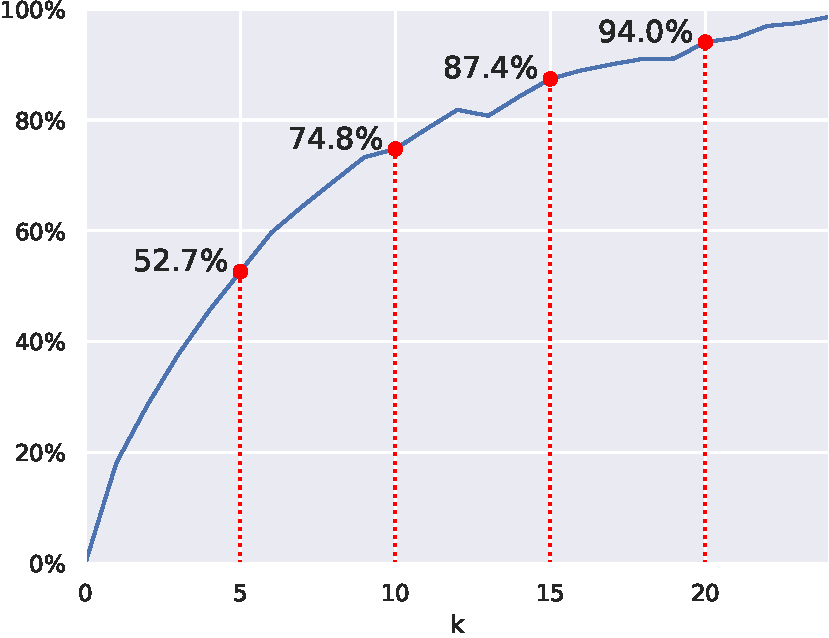
\includegraphics[height=45mm]{./images/graphs/12_hybrid_common_Decentraland_W-THU_normalize=True.pdf}
        \caption{Porcentaje de propuestas en común entre los dos recomendadores}
    \end{figure}
\end{frame}    

\begin{frame}{Métodos de fusión}
    \begin{figure}
        \centering
        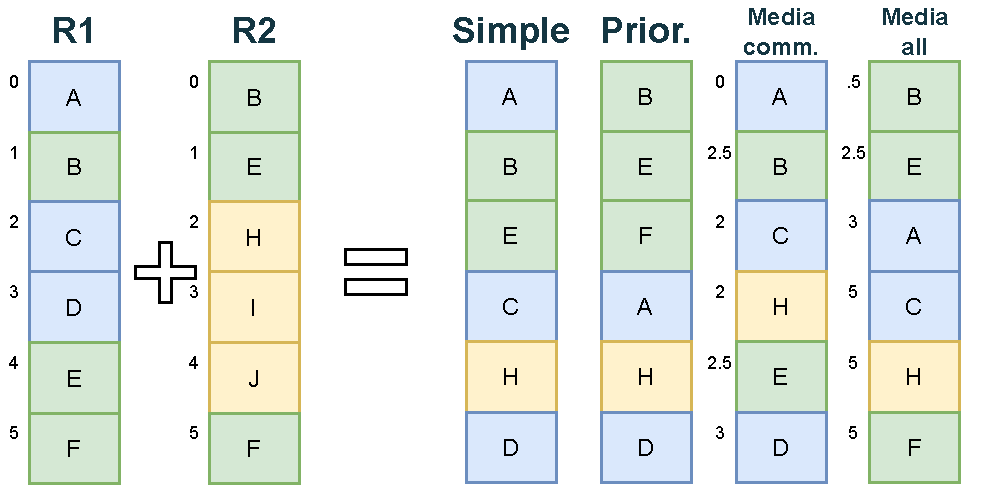
\includegraphics[height=45mm]{./images/diagrams/metodos-fusion.drawio.pdf}
        \caption{Distintos métodos de fusión utilizados}
    \end{figure}
\end{frame}

\begin{frame}{Resultados}
    \begin{figure}
        \centering
        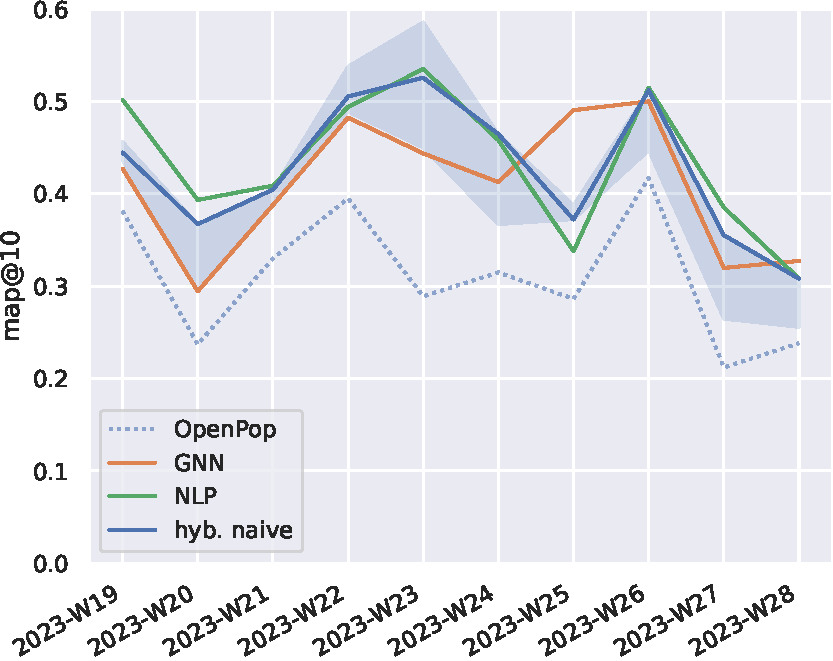
\includegraphics[height=45mm]{./images/graphs/12_hybrid_merge_results_folds_Decentraland_W-THU_normalize=True_compare.pdf}
        \caption{Resultados en cada fold de los sistemas recomendadores}
    \end{figure}
\end{frame}